\documentclass[11pt]{article}
\usepackage{graphicx}
\author{Ryan Smith \& David Cronkite \\ \{ryansmit, cronkd\}@uw.edu}
\title{Graded Reader}

\begin{document}
\maketitle

The goal of our app is to create a program that emulates a ``graded reader'' type book.  A graded reader is traditionally a text that is in L2 and along the margins or as footnotes has annotation on the vocabulary the writer of the graded reader believes the reader would have to look up in a dictionary at this point in their language learning.  The goal is that the reader can begin to read texts written in the L2 without the frustration of having to constantly go back and forwards between the text and a dictionary (especially if a dictionary might not help, as in a new grammar structure or an irregular word).  The ``graded'' part of graded reader is implying a course-like structure going from very low level language ability, with large amounts of word definitions given, to a point where only a select few words need to have the translation given.

Our goal is to create an app that can improve upon this concept by allowing each word to be looked up when clicked, as in figure \ref{words}. The idea is that the file providing the text will include this definition, making it context sensitive, and if not provided have it looked up in a dictionary, making it context insensitive.  Taking this a step further though, the user will also be able to select an entire sentence and have a translation provided for them, as in figure \ref{sentences}.  Again, the concept is that the text provider will ideally provide the translations, and if not provided then the app will use an external machine translation if possible.

\begin{figure}[h]
  \caption{Word definitions}
  \label{words}
  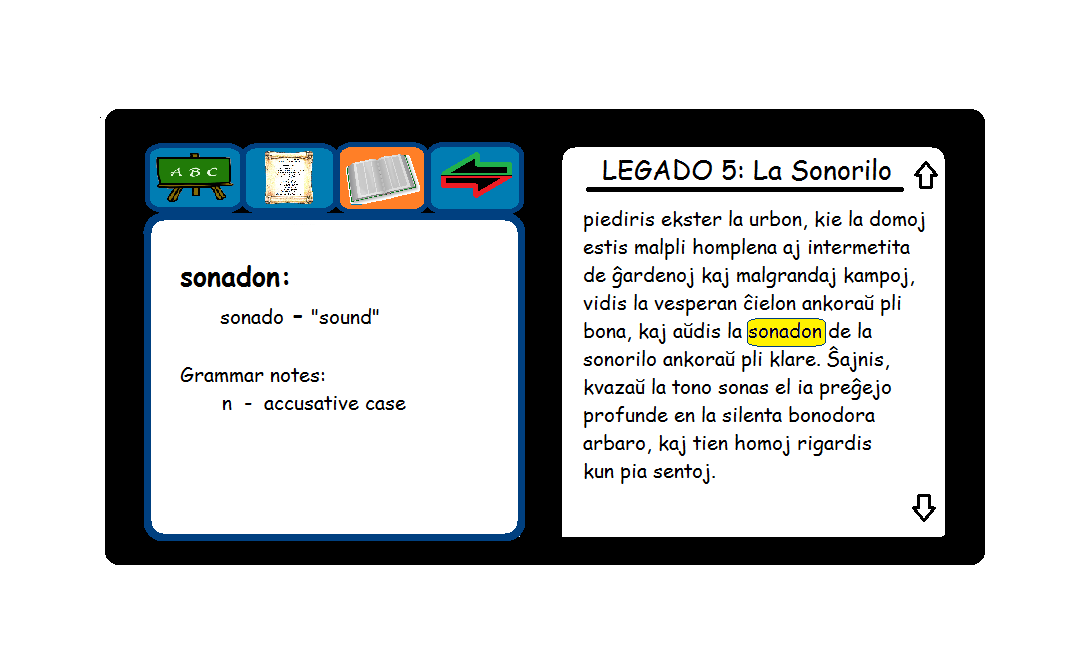
\includegraphics[scale=.5]{word_look_up.png}
\end{figure}

\begin{figure}[h]
  \caption{Sentence translation}
  \label{sentences}
  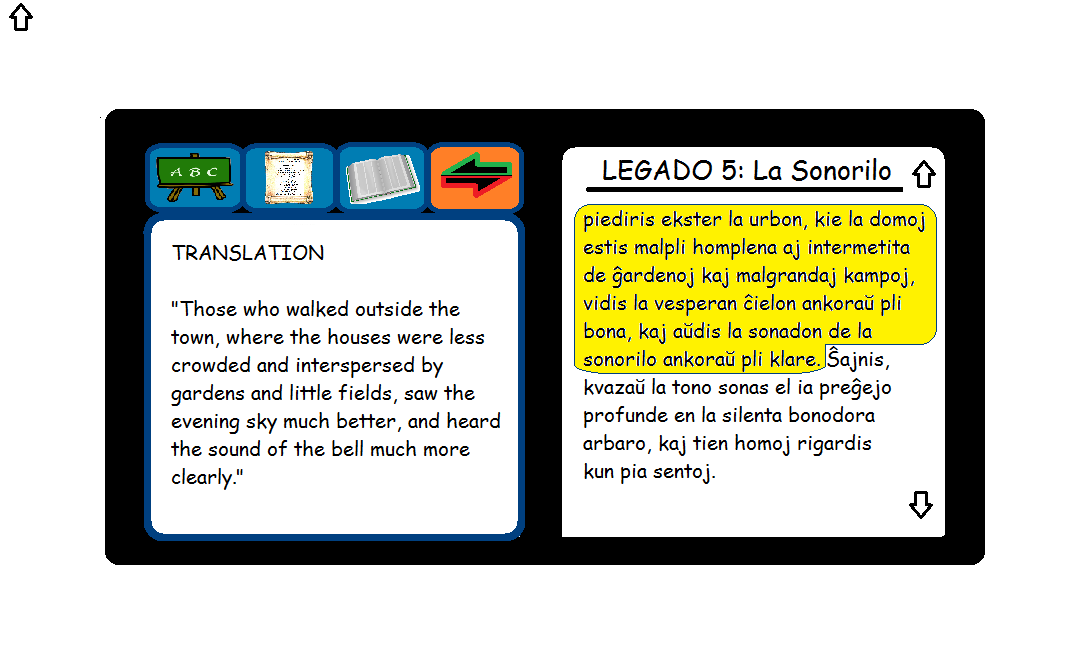
\includegraphics[scale=.5]{translate_tab.png}
\end{figure}

Besides just the dictionary look up, we would also like to have the text include a list of ``most important vocabulary'' that would provide the reader with the words most likely needing to be looked up, just like a traditional graded reader would (see figure \ref{vocab}). This will allow the reader to not have to be constantly clicking words, if the text provider already knows a word is likely to cause problems.

\begin{figure}[h]
  \caption{Vocabulary List}
  \label{vocab}
  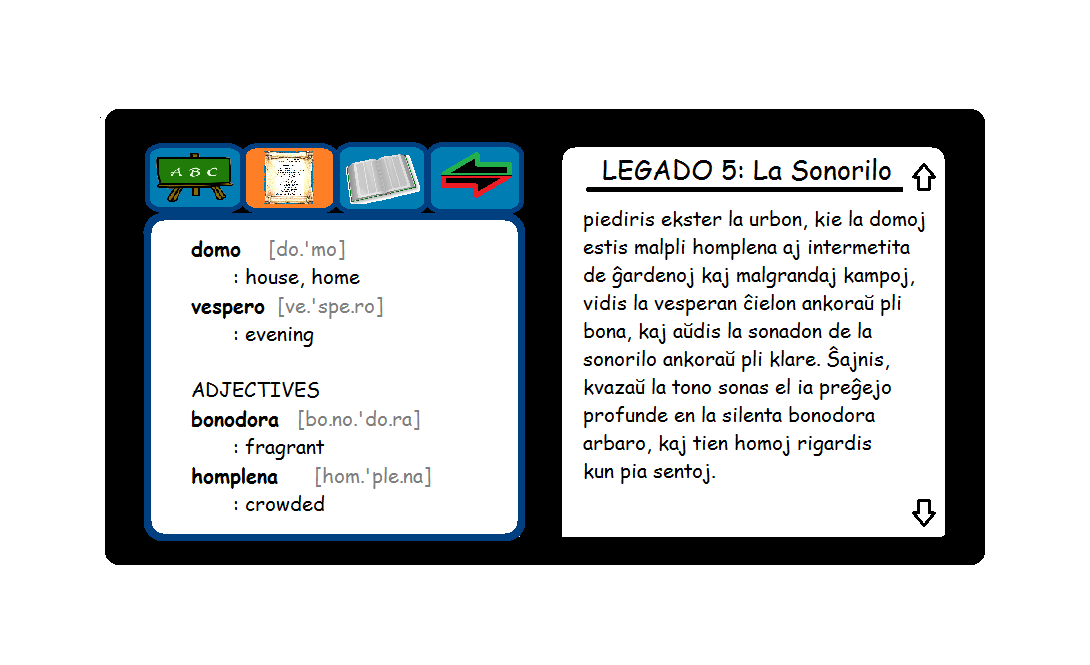
\includegraphics[scale=.5]{vocabulary_list.png}
\end{figure}

Something that would allow for a collection of these texts to become a full language learning tool on it's own is to include a section that discusses new grammatical content of a text, which a reader could peruse before attempting to read the text.  A possible concept for this is in figure \ref{grammar}.

\begin{figure}[h]
  \caption{New grammar information}
  \label{grammar}
  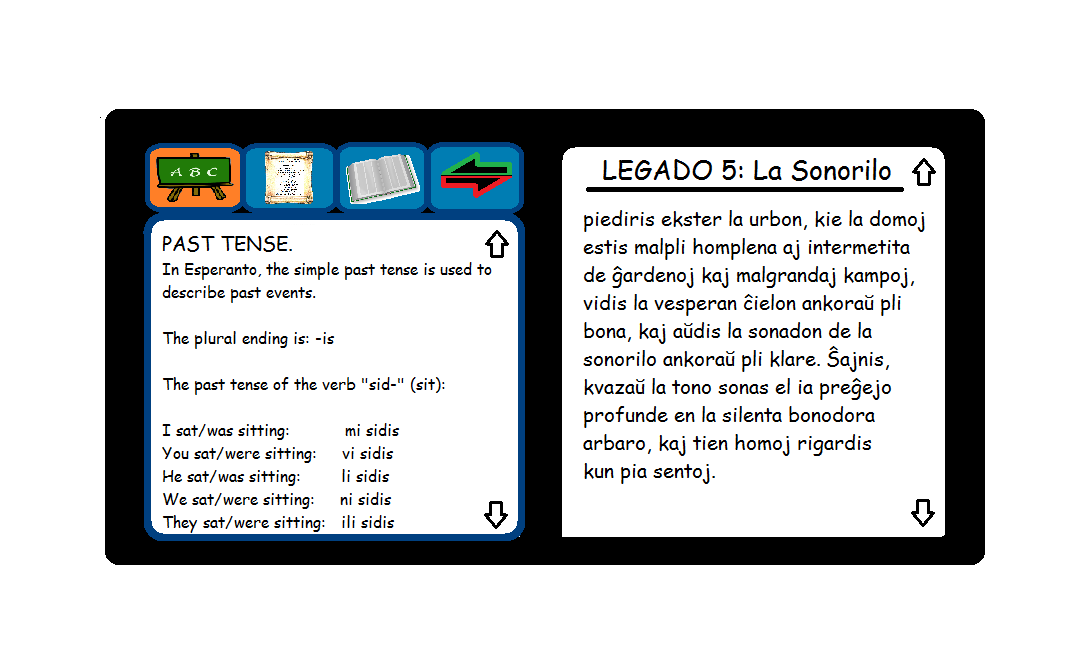
\includegraphics[scale=.5]{grammar_tab.png}
\end{figure}

While the SDK provides the main components we'll need (text views), we'll need to create the tabbed interface for the landscape view, as well as come up with some useful portrait view, and also create the linking between clicking on either a sentence or a word and have the appropriate translation appear in the window on the left.  We'll also need the ability to do dictionary look ups and automatic translations for when the data file doesn't provide these. The data we'll need is texts which include information about the grammar, the new vocab, the context-sensitive word meanings, and possible sentence-level translations. We'll have to create these files ourselves, but the end goal is to create an open file format (probably XML) and a desktop application which anyone can use to generate new content.

\end{document}
